\documentclass[12pt]{scrartcl}
\usepackage[sexy]{james}
\usepackage[noend]{algpseudocode}
\setlength {\marginparwidth}{2cm}
\usepackage{answers}
\usepackage{array}
\usepackage{tikz}
\newenvironment{allintypewriter}{\ttfamily}{\par}
\usepackage{listings}
\usepackage{xcolor}
\usetikzlibrary{arrows.meta}
\usepackage{color}
\usepackage{mathtools}
\newcommand{\U}{\mathcal{U}}
\newcommand{\E}{\mathbb{E}}
\usetikzlibrary{arrows}
\Newassociation{hint}{hintitem}{all-hints}
\renewcommand{\solutionextension}{out}
\renewenvironment{hintitem}[1]{\item[\bfseries #1.]}{}
\renewcommand{\O}{\mathcal{O}}
\declaretheorem[style=thmbluebox,name={Chinese Remainder Theorem}]{CRT}
\renewcommand{\theCRT}{\Alph{CRT}}
\setlength\parindent{0pt}
\usepackage{sansmath}
\usepackage{pgfplots}

\usetikzlibrary{automata}
\usetikzlibrary{positioning}  %                 ...positioning nodes
\usetikzlibrary{arrows}       %                 ...customizing arrows
\newcommand{\eqdef}{=\vcentcolon}
\newcommand{\tr}{{\rm tr\ }}
\newcommand{\im}{{\rm Im\ }}
\newcommand{\spann}{{\rm span\ }}
\newcommand{\Col}{{\rm Col\ }}
\newcommand{\Row}{{\rm Row\ }}
\newcommand{\dint}{\displaystyle\int}
\newcommand{\dt}{\ {\rm d }t}
\newcommand{\PP}{\mathbb{P}}
\newcommand{\horizontal}{\par\noindent\rule{\textwidth}{0.4pt}}
\usepackage[top=3cm,left=3cm,right=3cm,bottom=3cm]{geometry}
\newcommand{\mref}[3][red]{\hypersetup{linkcolor=#1}\cref{#2}{#3}\hypersetup{linkcolor=blue}}%<<<changed

\tikzset{node distance=4.5cm, % Minimum distance between two nodes. Change if necessary.
         every state/.style={ % Sets the properties for each state
           semithick,
           fill=cyan!40},
         initial text={},     % No label on start arrow
         double distance=4pt, % Adjust appearance of accept states
         every edge/.style={  % Sets the properties for each transition
         draw,
           ->,>=stealth',     % Makes edges directed with bold arrowheads
           auto,
           semithick}}


% Start of document.
\newcommand{\sep}{\hspace*{.5em}}

\pgfplotsset{compat=1.18}
\begin{document}
\title{MATH403: Homework 2}
\author{James Zhang\thanks{Email: \mailto{jzhang72@terpmail.umd.edu}}}
\date{\today}

\definecolor{dkgreen}{rgb}{0,0.6,0}
\definecolor{gray}{rgb}{0.5,0.5,0.5}
\definecolor{mauve}{rgb}{0.58,0,0.82}

\lstset{frame=tb,
  language=Java,
  aboveskip=3mm,
  belowskip=3mm,
  showstringspaces=false,
  columns=flexible,
  basicstyle={\small\ttfamily},
  numbers=left,
  numberstyle=\tiny\color{gray},
  keywordstyle=\color{blue},
  commentstyle=\color{dkgreen},
  stringstyle=\color{mauve},
  breaklines=true,
  breakatwhitespace=true,
  tabsize=3
}

\maketitle

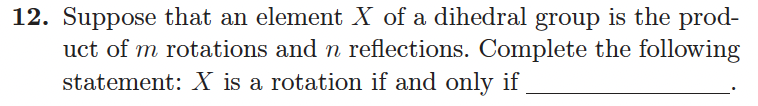
\includegraphics[width=14cm]{12.png}

\[ X \text{ is a rotation if and only if } \textbf{$n$ is even}\]

\begin{proof}[Solution]
  Observe the Cayley table for $D_4$ from the textbook as reference, but we will generalize for all 
  dihedral groups. 

  \begin{center}
    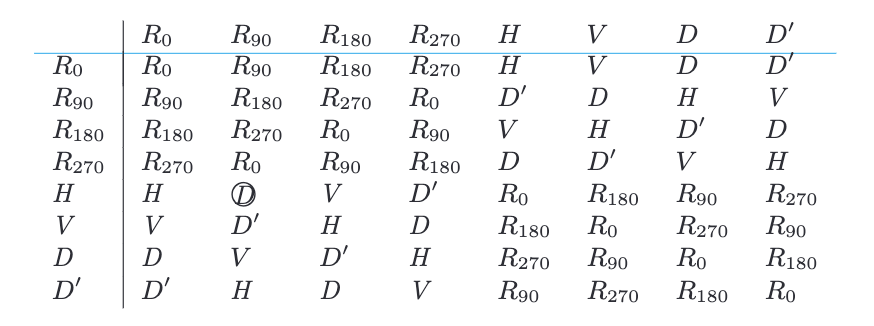
\includegraphics[width=10cm]{d4table.png}
  \end{center}

  Let's first consider the value $m$, the number of rotations. Trivially, $1$ rotation 
  is a rotation. From the table, we see that $2$ rotations is still a rotation, and this holds for all 
  dihedral groups, so if $n=0$, then $X$ is a rotation for all $m$. Now let's consider 
  nonzero $n$. If $n$ is odd, either a singular reflection or a sequence of reflections and rotations, 
  then $X$ will be a reflection. However, an even number of reflections results in a rotation. Therefore, 
  $X$ is a rotation if and only if $n$ is even. 
\end{proof}

\newpage 

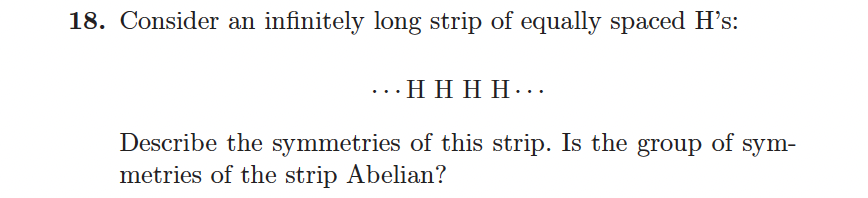
\includegraphics[width=14cm]{18.png}

\begin{proof}
  Recall that a group is Abelian (or commutative) if $ab = ba$ for all choices of 
  group elements $a, b$. Let us enumerate the infinite strip of $H$'s for the sake of determining if the strip is Abelian.
  \begin{align}
    \cdots \ \ H_{-2} \ \ H_{-1} \ \ H_0 \ \ H_1 \ \ H_2 \ \ \cdots
  \end{align}
  Visually, ignoring the enumerations, if you translate the strip left or right $n$ units or even reflect 
  the strip horizontally, the strip will still appear the same, but let's take a closer look with the aid of 
  our enumerations. Let us define two transformations: $T(n)$, which is a translation $n$ units such that positive is to the right 
  and negative is to the left (analagous to a real number line), and $R$, a horizontal reflection. We will show that 
  $T(1) \ R$ and $R \ T(1)$ do not result in the same final state, and thus the strip is not Abelian. 

  \hfill

  Case 1: $T(1) \ R$. The reflection $R$ turns (1) into 
  \begin{align*}
    \cdots \ \ H_{2} \ \ H_{1} \ \ H_0 \ \ H_{-1} \ \ H_{-2} \ \ \cdots
  \end{align*}
  and then the translation turns this into 
  \begin{align}
    \cdots \ \ H_{3} \ \ H_{2} \ \ H_1 \ \ H_{0} \ \ H_{-1} \ \ \cdots
  \end{align}

  \hfill

  Case 2: $R \ T(1)$. The translation turns (1) into 
  \begin{align*}
    \cdots \ \ H_{-3} \ \ H_{-2} \ \ H_{-1} \ \ H_0 \ \ H_1 \ \ \cdots
  \end{align*}
  and then the reflection would result in
  \begin{align}
    \cdots \ \ H_{1} \ \ H_{0} \ \ H_{-1} \ \ H_{-2} \ \ H_{-3} \ \ \cdots
  \end{align}
  and clearly, (2) and (3) are not the same final state, and so the strip is not Abelian.
\end{proof}

\newpage 

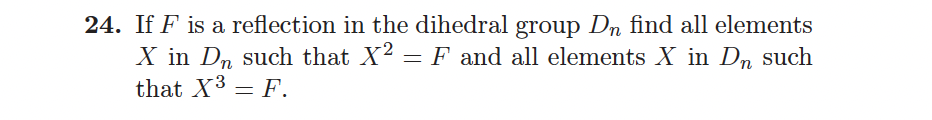
\includegraphics[width=14cm]{24.png}

\begin{proof}
  For the following, let $F$ be a \textit{reflection} in $D_n$.
  \begin{enumerate}[(i)]
    \item First, let us find all elements $X$ in $D_n$ such that $X^2 = F$. Note that any rotation followed by the same rotation results a new rotation, so there are 
    no rotations in the set $X$. Furthermore, given any reflection, applying that same reflection twice over results in $R_0$, which 
    cannot be the reflection $F$. Therefore, $X = \emptyset$, the empty set.
    \item For all elements $X$ in $D_n$ such that $X^3 = F$, we apply similar logic. Any rotation applied three 
    times successively will result in an new rotation, so there are no rotations in $X$. Now onto reflections. 
    Equipped with the fact that applying the same reflection twice back to back results in $R_0$, applying the same reflection 
    the third time would be equivalent to have only applying the reflection once. Therefore, for any given $F$, $X$ only 
    contains one element: $F$. $X = \{F\}$.
  \end{enumerate}
\end{proof}

\newpage 

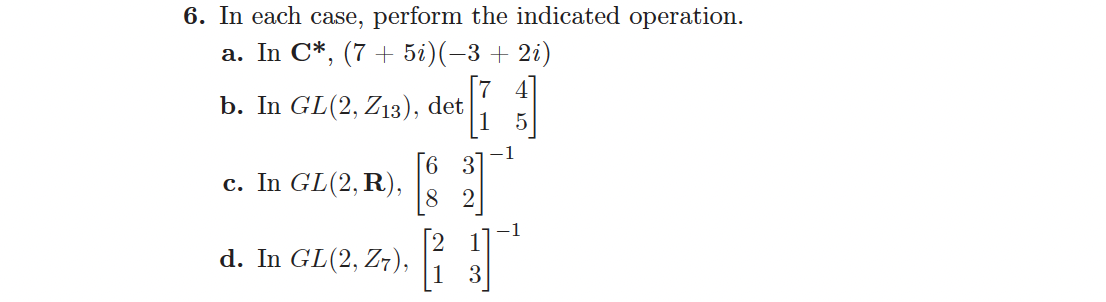
\includegraphics[width=14cm]{6.png}

\begin{proof}
  \hfill

  \begin{enumerate}[a.]
    \item $(7 + 5i)(-3 + 2i) = -21 + 14i - 15i + 10i^2 = -31 - i$
    \item $35 - 4 = 31$ but we need this in $Z_{13}$ so $31 \text{ mod } 13 = 5$ and so
    the determinant in $GL(2, Z_{13})$ is $5$.
    \item Using the formula for inverse of a $2\times 2$ matrix, 
    \[\begin{bmatrix}
      6 & 3\\ 8 & 2
    \end{bmatrix}^{-1} = \begin{bmatrix}
      -\frac{1}{6} & \frac{1}{4}\\
      \frac{2}{3} & -\frac{1}{2}
    \end{bmatrix}\]
    whcih is already in $GL(2, \RR)$ and so we are done.
    \item We have to be more careful with this example. Recall that the inverse of a $2 \times 2$ matrix $M$ is 
    given by 
    \[\begin{bmatrix}
      a & b\\ c & d
    \end{bmatrix}^{-1} = \frac{1}{\det M} \begin{bmatrix}
      d & -b \\ -c & a
    \end{bmatrix}\]
    The determinant of our matrix is $2(3) - 1(1) = 5$. The modular mutliplicative inverse of $t$ in 
    $Z_7$ is $3$. Therefore, we now compute 
    \[3 \begin{bmatrix}
      3 & -1\\ -1 & 2
    \end{bmatrix} = \begin{bmatrix}
      9 & -3\\
      -3 & 6
    \end{bmatrix} \implies \begin{bmatrix}
      2 & 4\\ 4 & 6
    \end{bmatrix} \in Z_7\]
    and we are done.
  \end{enumerate}
\end{proof}

\newpage 


\includegraphics[width=14cm]{10.png}

\begin{proof}
  Recall that $U(n)$ is the set of all positive integers less than $n$ and relatively prime to $n$. 
  Thus, $U(20) = \{1, 3, 7, 9, 11, 13, 17, 19\}$. For inverses, note that
  \begin{itemize}
    \item $1 * 1 \equiv 1 (\text{mod } 20)$, so $1$ is its own inverse
    \item $3 * 7 \equiv 21 \equiv 1 (\text{mod} 20)$, so $3$ and $7$ are inverses of each other
    \item $9 * 9 \equiv 81 \equiv 1 (\text{mod } 20)$, so $9$ is its own inverse
    \item $11 * 11 \equiv 121 \equiv 1 (\text{mod } 20)$, so $11$ is its own inverse
    \item $13 * 17 \equiv 221 \equiv 1 (\text{mod } 20)$, so $13$ and $17$ are inverses of each other
    \item $19 * 19 \equiv 361 \equiv 1 (\text{mod } 20)$, so $19$ is its own inverse.
  \end{itemize}
\end{proof}

\newpage 


\includegraphics[width=14cm]{36.png}

\begin{proof}
  
\hfill

\begin{enumerate}[(i)]
  \item First let us prove that $(ab)^2 = a^2b^2$ if and only if $ab = ba$. 
  
  $\Longrightarrow$ Assume $(ab)^2 = a^2b^2$. We want to show that $ab = ba$.
  Taking our given statement and expanding, we obtain
  \[(ab)(ab) = aabb\]
  Now by associativity of groups, 
  \[a(ba)b = a(ab)b\]
  By the inverses of groups, we apply 
  \[a^{-1} a (ba) b b^{-1} = a^{-1} a(ab) b b^{-1} \implies e(ba)e = e(ab)a \implies ba = ab\]
  Therefore, any group with this property must be Abelian. 

  $\Longleftarrow$ Now assume the group is Abelian, so $ab = ba$. We want to show that $(ab)^2 = a^2b^2$. 
  \[ba = ab \implies aba = aab \implies abab = aabb\]
  By associativity of groups, 
  \[abab = aabb \implies (ab)(ab) = (aa)(bb) \implies (ab)^2 = a^2b^2\]

  \item Now let us prove that $(ab)^{-2} = b^{-2}a^{-2}$ if and only if $ab = ba$.
  
  $\Longrightarrow$ Assume that $(ab)^{-2} = b^{-2}a^{-2}$. We want to show that $ab = ba$. Multiply 
  both sides by $(ab)^2$ on the left
  \[(ab)^2 (ab)^{-2} = (ab)^2 b^{-2}a^{-2} \implies e = (ab)^2b^{-2}a^{-2}\]
  Multiply both sides by $a^2$ on the right to get 
  \[a^2 = (ab)^2b^{-2} a^{-2} a^2 \implies a^2 = (ab)^2 b^{-2} e \implies a^2 = (ab)^2b^{-2}\]
  Multiply both sides on the right by $b^2$ and this yields 
  \[a^2b^2 = (ab)^2e \implies a^2b^2 = (ab)^2\]
  From here, we apply the same proof in part $i$, and we have shown that $ab = ba$.

  $\Longleftarrow$ Assume $ab = ba$, we want to show that $(ab)^{-2} = b^{-2}a^{-2}$. Furthermore, note 
  the property $(ab)^{-1} = b^{-1}a^{-1}$ and we can quickly show this because $(ab)b^{-1}a^{-1} = a(bb^{-1})a^{-1} = e$. Now observe that 
  \[(ab)^{-2} = ((ab^{-1}))^2 = (b^{-1}a^{-1})^2 = (b^{-1}a^{-1})(b^{-1}a^{-1})\]
  Since we have commutativivity, we can rearrange such that 
  \[(ab)^{-2} = (b^{-1}b^{-1})(a^{-1}a^{-1}) = b^{-2}a^{-2}\]
  and so $(ab)^{-2} = b^{-2}a^{-2}$ as desired.
\end{enumerate}

\end{proof}

\newpage 

\end{document}

